\section{Visión general}

El sistema se organiza en dos partes principales. Por un lado, la
computadora, que edita y traduce el programa y presenta los
resultados. Por el otro lado, la FPGA, que almacena y ejecuta
la imagen y responde con observaciones. La comunicación se realiza por
el puente USB-UART de la placa.

La figura~\ref{fig:sistema-general} resume la topología del sistema.
La computadora se conecta con la FPGA a través del puente USB-UART;
el núcleo UART entrega los bytes al controlador de protocolo, que
coordina la carga y la ejecución con el procesador. El serializador
de respuestas devuelve las observaciones por el mismo enlace UART.

\begin{figure}[H]
  \centering
  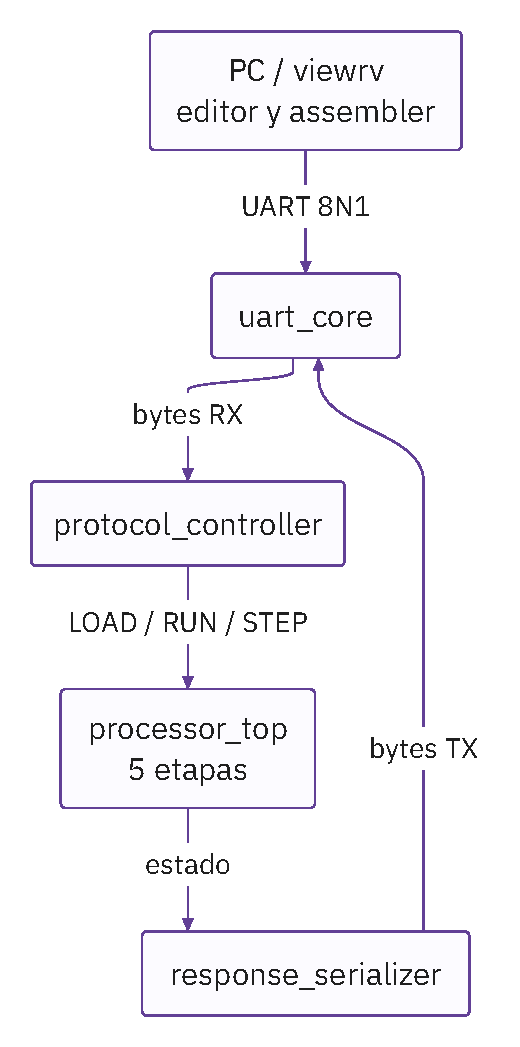
\includegraphics[width=0.34\textwidth]{sistema-general.pdf}
  \caption{Topología del sistema.}
  \label{fig:sistema-general}
\end{figure}

\section{Jerarquía y responsabilidades}

La jerarquía aprobada se resume en la tabla~\ref{tab:jerarquia}. El
inventario completo, con los 51 bloques del CPU y su ubicación, se
consulta en \doc{architecture/module_inventory.md}{Inventario de módulos}.

\begin{table}[H]
  \centering
  \small
  \begin{tabularx}{\textwidth}{L{4.8cm}Y}
    \toprule
    \textbf{Módulo} & \textbf{Responsabilidad} \\
    \midrule
    \code{basys3_top} & Adapta el sistema a la Basys 3: expone los cuatro
    puertos físicos, selecciona el perfil \code{MEMORY_PROFILE},
    instancia el Clocking
    Wizard (MMCM/BUFG de 100 a 50 MHz con \code{locked}), distribuye el
    \code{reset_sync} común y conecta \code{system_top}. \\ \addlinespace
    \code{system_top} & Integra el sistema funcional: conecta
    \code{uart_core}, \code{protocol_controller},
    \code{response_serializer} y \code{processor_top}, y distribuye clock,
    reset, capacidades de memoria y señales de observación. \\ \addlinespace
    \code{processor_top} & Contiene el procesador y sus servicios: pipeline de
    cinco etapas, cuatro registros interetapa, RF, IMEM/DMEM, forwarding y
    hazards, \code{execution_control}, \code{loader} y
    \code{session_preparation}; expone PC, RF, latches, fault y memoria
    utilizada para Debug. \\ \addlinespace
    \code{uart_core} & Implementa el transporte serie: sincroniza RX, genera
    el tick de sobremuestreo 16$\times$ para RX/TX, recibe y valida tramas
    8N1, transmite bytes y conserva FIFO independientes de cuatro bytes para
    recepción y transmisión. \\ \addlinespace
    \code{protocol_controller} & Interpreta \code{LOAD}, \code{RUN},
    \code{STEP}, \code{RESET} y \code{CHECK_READY}; valida tamaño y secuencia,
    coordina carga y preparación, solicita \code{RUN}/\code{STEP}, administra
    Debug, timeouts, silencio y recuperación. \\ \addlinespace
    \code{response_serializer} & Captura el descriptor del controlador y
    produce la respuesta completa: cabecera, contexto, banco de registros,
    latches y lista de DMEM. Lee el estado retenido para el snapshot y señala
    el fin físico del mensaje, incluido el último Stop. \\
    \bottomrule
  \end{tabularx}
  \caption{Jerarquía principal y responsabilidades.}
  \label{tab:jerarquia}
\end{table}

El CPU se distribuye en 51 bloques funcionales: 23 se implementan
como módulos específicos y 28 como lógica o estado local dentro de
una etapa o del top.

\section{Organización del procesador}

El procesador es un pipeline \emph{in-order} de cinco etapas. Cada instrucción
avanza como máximo una etapa por ciclo efectivo. La figura~\ref{fig:pipeline}
muestra el recorrido y la tabla~\ref{tab:etapas} resume la función de cada
etapa.

\begin{figure}[H]
  \centering
  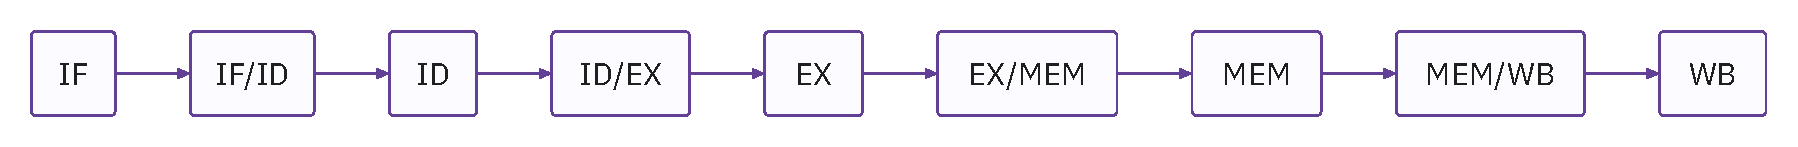
\includegraphics[width=\textwidth]{pipeline.pdf}
  \caption{Etapas y registros interetapa del procesador.}
  \label{fig:pipeline}
\end{figure}

\begin{table}[H]
  \centering
  \small
  \begin{tabularx}{\textwidth}{L{1.4cm}Y}
    \toprule
    \textbf{Etapa} & \textbf{Función principal} \\
    \midrule
    IF & Mantiene el PC, lee IMEM, valida la búsqueda y forma el candidato de
    fault de fetch. \\ \addlinespace
    ID & Decodifica la instrucción, lee el banco de registros, genera el
    inmediato, aplica el bypass \tech{WB}$\rightarrow$\tech{ID} y detecta
    load-use e instrucciones ilegales. \\ \addlinespace
    EX & Selecciona operandos con forwarding, ejecuta la ALU, calcula
    direcciones, resuelve branches y jumps, y confirma faults propios y
    la instrucción \code{halt}. \\ \addlinespace
    MEM & Accede a DMEM, selecciona y extiende loads, aplica la máscara de
    stores y forma el valor de writeback. \\ \addlinespace
    WB & Escribe el banco de registros y genera los controles de bypass hacia
    ID. \\
    \bottomrule
  \end{tabularx}
  \caption{Responsabilidad de cada etapa.}
  \label{tab:etapas}
\end{table}

Los cuatro registros interetapa conservan la validez y los campos que la etapa
siguiente necesita; su organización y la semántica de validez se detallan en la
sección~\ref{sec:registros-interetapa}.

\section{Conjunto de instrucciones}

El decoder implementa 32 instrucciones de \tech{RV32I} y la palabra exacta de
\code{halt}. A continuación se resumen las familias de instrucciones.

\begin{table}[H]
  \centering
  \small
  \begin{tabularx}{\textwidth}{L{3.2cm}Y}
    \toprule
    \textbf{Familia} & \textbf{Instrucciones} \\
    \midrule
    Registro & \code{ADD}, \code{SUB}, \code{SLL}, \code{SLT}, \code{SLTU},
    \code{XOR}, \code{SRL}, \code{SRA}, \code{OR}, \code{AND} \\
    \addlinespace
    Inmediato & \code{ADDI}, \code{SLTI}, \code{SLTIU}, \code{XORI},
    \code{ORI}, \code{ANDI}, \code{SLLI}, \code{SRLI}, \code{SRAI} \\
    \addlinespace
    Loads & \code{LB}, \code{LH}, \code{LW}, \code{LBU}, \code{LHU} \\
    \addlinespace
    Stores & \code{SB}, \code{SH}, \code{SW} \\
    \addlinespace
    Flujo & \code{BEQ}, \code{BNE}, \code{JAL}, \code{JALR} \\
    \addlinespace
    Inmediato superior & \code{LUI} \\
    \addlinespace
    Terminación & \code{halt} = \code{0x0000000B} \\
    \bottomrule
  \end{tabularx}
  \caption{Subconjunto de instrucciones implementado.}
  \label{tab:isa}
\end{table}

\code{halt} se codifica con la palabra exacta \code{0x0000000B}. Los bits
31:7 son cero y los bits 6:0 forman el opcode \code{0001011}, que el mapa de
RISC-V User-Level ISA V2.2 reserva para la extensión \code{custom-0}. La
instrucción no tiene operandos y no escribe el banco de registros ni DMEM.

La codificación se adoptó para disponer de una terminación explícita sin
reutilizar una instrucción estándar con otra semántica. Usar \code{EBREAK}
habría mezclado la finalización normal con una excepción de breakpoint, y
reservar \code{0x00000000} habría confundido una memoria sin programar con un
\code{halt} intencional. El espacio \code{custom-0} permite introducir la
instrucción sin colisionar con RV32I, y la palabra completa distingue
\code{halt} de cualquier otra codificación custom.

Toda instrucción distinta de las codificaciones admitidas produce
\code{ILLEGAL_INSTRUCTION}. La legalidad se comprueba en ID; la memoria no
decide si una palabra es una instrucción válida.

\section{Separación entre datos y control}

El camino de datos o \emph{datapath} reúne los bloques que almacenan y
procesan la información: el PC, el banco de registros, las memorias, la ALU,
los sumadores y los multiplexores. Por estos bloques circulan las
instrucciones, sus operandos y los resultados. Las señales de control indican
qué operación realizar, qué entrada elegir en cada multiplexor y cuándo
actualizar el PC y los registros interetapa.

El control se distribuye entre los siguientes bloques:

\begin{itemize}
  \item \textbf{Decoder:} identifica la operación que solicita cada instrucción
  y genera sus señales de control.
  \item \textbf{Unidad de forwarding:} selecciona resultados de instrucciones
  anteriores para que EX pueda utilizarlos antes de que se escriban en el
  banco de registros.
  \item \textbf{Detector de \code{load-use}:} identifica cuándo una instrucción
  debe esperar porque necesita el dato de un load que aún no está disponible.
  \item \textbf{\code{Flow Control}:} determina si corresponde cambiar el flujo
  de ejecución y selecciona qué dirección de destino utilizar.
  \item \textbf{Comprobadores de fault:} detectan errores en las instrucciones
  y en los accesos a memoria.
  \item \textbf{\code{Pipeline Hazard Control}:} reúne esas condiciones y
  decide qué instrucciones pueden continuar, cuáles deben esperar y cuáles
  se deben descartar.
\end{itemize}

En cada ciclo habilitado por \code{cpu_cycle_fire},
\code{Pipeline Hazard Control} elige una sola acción. Fuera del modo de
drenado, aplica la primera condición que se cumpla en este orden:

\begin{enumerate}
  \item Fault de la instrucción en EX.
  \item \code{halt} en EX.
  \item Cambio de flujo resuelto en EX.
  \item Fault de la instrucción en ID.
  \item Espera por una dependencia \code{load-use}.
  \item Avance normal, si no se cumple ninguna de las condiciones anteriores.
\end{enumerate}

Los eventos de EX tienen prioridad sobre los de ID porque corresponden a una
instrucción anterior en el programa. Además, un fault de la propia instrucción
impide aplicar sus otros efectos.

Durante el drenado (\code{drain_mode}), el control deja de incorporar
instrucciones nuevas y permite que terminen las que siguen activas. Para este
modo hay dos acciones adicionales: avanzar o esperar por una dependencia
\code{load-use}. En total se definen ocho acciones, cuyos efectos sobre el PC
y los registros interetapa se detallan en la tabla~\ref{tab:acciones} y en
\doc{architecture/cpu/control_and_hazards.md}{Control y hazards}. Si
\code{cpu_cycle_fire} vale cero, no se aplica ninguna de ellas.

\section{Debug y observación}

Debug permite consultar el estado que la ejecución ya dejó registrado, sin
modificarlo ni agregar ciclos al procesador. La observación combina dos tipos
de información:

\begin{itemize}
  \item \textbf{Estado arquitectónico:} PC, contador de ciclos, causa y PC de
  fault, banco de registros y bytes de DMEM que fueron utilizados.
  \item \textbf{Estado del pipeline:} validez y contenido de los registros
  \code{IF/ID}, \code{ID/EX}, \code{EX/MEM} y \code{MEM/WB}. Estos registros
  permiten saber qué instrucciones todavía están en vuelo y qué datos llevan
  entre etapas.
\end{itemize}

El controlador de protocolo retiene la CPU mientras se arma la respuesta. En
ese intervalo selecciona, de manera alternada, las direcciones de lectura del
banco de registros y de DMEM. El serializador toma esas lecturas y los campos
de los registros interetapa, y los transmite en el orden fijado por el
protocolo. Así, todos los campos del snapshot corresponden al mismo estado
observado.

El snapshot contiene:

\begin{itemize}
  \item el estado global de la sesión y la validez de la imagen cargada;
  \item el PC y el contador de ciclos;
  \item la causa y el PC del fault, cuando existe;
  \item los 32 registros del banco de registros;
  \item los campos definidos de los cuatro registros interetapa;
  \item la cantidad de bytes utilizados de DMEM y la lista de sus direcciones
  y valores.
\end{itemize}

La observación se realiza después del último ciclo autorizado, por ejemplo,
después de un \code{STEP} o al finalizar un \code{RUN}.

La estructura y los códigos se detallan en \doc{protocol.md}{Protocolo UART} y en
\doc{architecture/debug/debug_architecture.md}{Arquitectura de Debug}.
